\providecommand{\main}{..}
\documentclass[\main/main.tex]{subfiles}

\begin{document}

\lesson{9}{28/10/20}
From now on we will consider $\mean{X}_0=0$ in order to simplify equations: in this way the relation (\ref{eq:wow}) can be rewritten as
\begin{equation}
    \mean{x(t)}=\beta h [\mean{X(t)X(0)}]
    \label{eq:wow2}
\end{equation}
where the relevance of this equation is that on the left hand side we see a non equilibrium relaxation to the final equilibrium value while on the right hand side  we see the behaviour of the average auto-correlation function of the observable $X$. the two quantities decay the same way in the limit of $\beta h<<1$ i.e. when linear response theory is valid. \\

Now we want to generalize (\ref{eq:wow2}) in the case of a generic perturbation $h(t)$.
We will start by defining a very important quantity, which is the \textbf{response function} $\Xi(t,t')$:
\begin{equation}
    \mean{X(t)}=\int dt'\Xi(t,t')h(t')
    \label{eq:importance}
\end{equation}
In principle the response function is a function of $t,t'$ but in the context of LRT it can be expressed as a function of $(t-t')$:
\begin{numcases}{\Xi(t,t') = \,}
\Xi(t-t') & if $t'<t$ \\
0 & if $t'>t$ (Because we want causality to hold.)
\end{numcases}
The response function tells how the system respond to the presence of a perturbation at previous time (so $t'$ needs to be smaller than $t$).

How do we determine $\Xi$? The trick is to consider the equation that we already derived for the previous specific case and it will allow us to derive the response function for the generic case: note that the importance of equation (\ref{eq:importance}) is given by the fact that when we know the response function then we can compute the non-equilibrium average of the observable $X$ for \textit{any} external perturbation $h(t)$. \\

In the case represented in Figure \ref{fig:pert} we get:
\begin{align}
    \int_{-\infty}^{0}dt'\Xi(t-t') \overset{\tau=t-t'}{=}&\int_{t}^{+\infty}d\tau \Xi(\tau)\overset{(\ref{eq:wow2})}{=}\frac{\mean{X(t)}}{h}=\beta \mean{X(t)X(0)}_0 \\
    \int_{t}^{+\infty}\Xi(\tau)d\tau = &\beta \mean{X(t)X(0)}_0
\end{align}

In this way we are able to express the response function in terms of equilibrium averages (of the A-C function). 

Now, if we derive with respect to time, we get an explicit equation for the response function:
\begin{equation}
    \Xi(t)=-\beta \theta(t) \frac{d}{dt}\mean{X(t)X(0)}_0
    \label{eq:RF}
\end{equation}
where $\theta(t)$ is the Heaviside step function. \\

From now one we need to play with Fourier Transforms in order to study the properties of $\Xi(\omega)$\footnote{We wrote $\Xi=\Xi(\omega)$ because now we are in the frequency domain.}:
\begin{equation}
    \Xi(\omega)=\int_{\mathbb{R}} e^{-i\omega t}\Xi(t)dt
\end{equation}

To clarify our FT convention we will define the IFT as:
\begin{equation}
    \Xi(t)=\int_{\mathbb{R}}\frac{d\omega}{2\pi}e^{i\omega t}\Xi(\omega)d\omega
\end{equation}

Notice that (\ref{eq:importance}) is a convolution so in Fourier space (FS) this expression will be a product of the two functions, therefore:
\begin{align}
    (\ref{eq:importance}) \overset{FS}{\longmapsto} \mean{X(\omega)}=h(\omega)\cdot\Xi(\omega)
\end{align}

and in other words in FS the out-of-equilibrium relaxation is just the product between the perturbation and the response function in FS. \\

Let's now rewrite equation (\ref{eq:RF}), which allows us to express the response function, in FS:
\begin{equation}
   (\ref{eq:RF}) \overset{FS}{\longmapsto} \Xi(\omega)=-\beta\int_{\mathbb{R}}\frac{d\omega'}{2\pi}\theta(\omega-\omega')\underbrace{i\omega'}_{=\frac{d}{dt}}C(\omega')
   \label{eq:response_c}
\end{equation}
where $C(t):=\mean{X(t)X(0)}_0$ to simply notation.

\subsubsection{Properties of $C(\omega)$}
The function $C(\omega)$ is known as \textit{power spectrum} and tells as a function of the frequency $\omega$ how the auto-correlation function is distributed. 'Power' is related to the power dissipated in the non-equilibrium relaxation.

Let's write the definition of the FT for $C(t)$:
\begin{align}
   C(\omega)=\int_{\mathbb{R}} dt \,e^{-i\omega t}C(t) \overset{(a)}{=} \lim_{T\to\infty}\frac{1}{T}\mean{|X_T(\omega)|^2}_0
   \label{eq:ftdef}
\end{align}

Where in (a) we used the \textbf{Wiener-Kinchin theorem}, which states that the power spectrum can be expressed as the limit for infinite $T$ of the equilibrium average of the square modulus of a function similar to a FT (in the limit of infinite $T$), namely:
\begin{equation}
    X_T(\omega)=\int_{-\frac{T}{2}}^{+\frac{T}{2}}dt\, e^{-i\omega t} X(t)
\end{equation}
In general the equilibrium average of $X_T$ does not admit a FT ($\mean{X(t)}_0 \notin \mathbb{L}^2$) so it diverges for $T\to\infty$ and this is why we have to consider the limit to get a converging quantity.

This expression shows that $C(\omega)\in \mathbb{R}$ and $C(\omega)\geq 0 \, \forall\, \omega$: from the FT definition in (\ref{eq:ftdef}) the A-C function could have been in general a complex number but actually is a real positive number for any frequency.

In order to make an example, let's consider a typical exponential decay (\textit{Lorentzian}), e.g.:
\begin{align}
    C(t) &=\frac{1}{\tau}\exp{-\frac{|t|}{\tau}} \,\, \forall \,t \in \mathbb{R}\\
    C(\omega) &= \underbrace{\frac{1}{1+i\omega}}_{\in\, \mathbb{C}}+\underbrace{\frac{1}{1-i\omega}}_{\in\,\mathbb{C}}=\underbrace{\frac{2}{1+\omega^2\tau^2}}_{\in \, \mathbb{R}}
\end{align}

Another interesting property of the power spectrum is that the A-C function is an even function of time, which implies that the power spectrum is also an even function of frequency: this is due to time translation invariance at equilibrium
\begin{equation}
    C(t)=C(-t) \Longleftrightarrow C(\omega)=C(-\omega)
\end{equation}
and due to time translation invariance at equilibrium, subtracting a $t$ term from the A-C function arguments,
\begin{equation}
    \mean{X(t)X(0)}_0=\mean{X(0)X(-t)}_0=C(-t)
\end{equation}

The IFT is defined as:
\begin{align}
    \Xi(t)=\frac{1}{2\pi}\int_{\mathbb{R}}\exp{i\omega t}\Xi(\omega)
    \label{eq:integral}
\end{align}
and the point is that it is useful to analytically extend the response function in the frequency domain to imaginary/complex frequencies: let's add to the frequency $\omega \in \mathbb{R}$ an imaginary part, namely
\begin{equation}
    z:=\omega-i\epsilon
\end{equation}
In order for the causality to hold i.e. $\Xi(t)=0$ for $t<0$, this implies that, extending the response function to a whole complex plain, $\Xi(z)$ needs to be \textit{analytic} $Im(z)<0$: this is due to the fact that if the response function is analytic then there are no poles in the lower half of the complex plain and therefore we can compute the integral (\ref{eq:integral}) in the frequency domain using\textit{ residues theorem}. Since there are no poles the exponential factor goes to zero if we are in the lower half of the complex plane (and this happens for negative times).

For negative times (if there are no poles in the lower half of the complex plain) then $\Xi(t)=0$ and causality holds.

Let's write an expression for the FT of $\theta(t)$:
\begin{align}
    \theta(\omega)&=\lim_{\epsilon\to0^+}\int_{0}^{+\infty} dt \exp (-(\epsilon + i\omega t))=\lim_{\epsilon\to0^+}\frac{1}{\epsilon+i\omega} = \\
    &=\pi\delta(\omega)-iPV(\frac{1}{\omega})
     \label{eq:HFT}
\end{align}

where $PV$ is the \textit{principal value}, namely:
\begin{equation}
    PV(\frac{1}{\omega}):=\lim_{\epsilon\to 0^+}[\int_{-\infty}^\epsilon \frac{\phi(\omega)}{\omega}d\omega+\int_{\epsilon}^{+\infty}\frac{\phi(\omega)}{\omega}d\omega]
\end{equation}

Formally the analytic continuation is a regularization and the fact that we see a $PV$ means that all equations we will write are in general valid in the distribution space and they only makes sense only if applied to test functions $\phi(\omega)$ \footnote{Appendix F of \textit{Livi and Politi} for more informations about the previous calculation.}. \\

Thanks to (\ref{eq:HFT}) we are now able to rewrite the definition of the response function (\ref{eq:response_c}) as
\begin{align}
    \Xi(\omega)=-\beta[\frac{i\omega}{2}C(\omega)+PV(\int_{-\infty}^{+\infty}\frac{d\omega'}{2\pi}\frac{\omega'}{\omega-\omega'}C(\omega'))]
\end{align}

using the fact that $C(\omega)$ is a real number: essentially the first term is the imaginary part, namely (remembering that $C(\omega)$ is even but it's multiplied by $\omega$):
\begin{equation}
    \boxed{\Xi^{\mathrm{I}}(\omega)=-\beta \frac{\omega}{2} C(\omega)} \longrightarrow \text{odd function of}\, \omega
    \label{eq:IM}
\end{equation}
while on the other hand the real part is:
\begin{equation}
    \boxed{\Xi^{\mathrm{R}}(\omega)=PV[ \int_{-\infty}^{+\infty} \frac{d \omega^{\prime}}{\pi} \frac{1}{\omega-\omega^{\prime}} \Xi^{\mathrm{I}}\left(\omega^{\prime}\right)]}
    \label{eq:RE}
\end{equation}
In this way we just need to know the imaginary part of the response function (or only the power spectrum) to know the real part (which is clearly an even function).

Written in this general way, equations (\ref{eq:IM}) and (\ref{eq:RE}) are one of the typical ways to express the \textit{fluctuation-dissipation theorem}, fluctuation because the power spectrum is related to the equilibrium average of the A-C function, while on the other hand the power spectrum is also related to energy dissipation in the non-equilibrium relaxation. \\

One can also express the fluctuation-dissipation theorem in a different way, called \textbf{Kramers-Kronig relation}, by writing the overall response function $Xi$ such that:
\begin{equation}
\boxed{\Xi(\omega)=\lim _{\epsilon \rightarrow 0^{+}} \int_{-\infty}^{+\infty} \frac{d \omega^{\prime}}{\pi} \frac{\Xi^{1}\left(\omega^{\prime}\right)}{\omega-\omega^{\prime}-i \epsilon}}
\end{equation}

Notice out that this expression is equivalent to the ones written above.

\subsection{Work done on a system by the perturbation}
Since we are out-of-equilibrium, we will talk how to use the previous formalism to compute the dissipation work: we are interested in the system energy $-h X$, which means that the work done by the field on the system comes with a '+' sign.

Formally, given that in general case, $h$ is a function of time we can write that:
\begin{equation}
W=\int_{-\infty}^{+\infty} d t \,h(t)\left\langle\frac{d X(t)}{d t}\right\rangle
\label{eq:int}
\end{equation}
where the average is a \textit{non-equilibrium average}; in the special case of periodic perturbations then the previous integral will be defined over a period of the perturbation.

In order to compute integral (\ref{eq:int}) we have to play with FT and the main point it is to use the Fluctuation - Dissipation theorem:
\begin{equation}
    \mean{X(t)}=\int_{-\infty}^{+\infty} dt'\Xi(t-t')h(t')
\end{equation}
We now consider the FT of all the quantities in the above expression ($h(t),h(t'),\Xi(t-t')$) and at the end we get (skipping the details of calculations):
\begin{equation}
    W=\int_{-\infty}^{+\infty}\frac{d\omega}{2\pi}i\omega\,\Xi(\omega)|h(\omega)|^2
\end{equation}

and since the perturbing field is real ($h(t) \in \mathbb{R}$) this implies that $h^*(\omega)=h(-\omega)$.

Since the result needs to be real, this implies that the only part that contributes to the integral is just the \textit{imaginary part} of the response function, so the dissipated work becomes:
\begin{equation}
    W=-\int_{-\infty}^{+\infty}\frac{d\omega}{2\pi}i\omega\Xi^{\text{I}}(\omega)|h(\omega)|^2
\end{equation}

and now we use the FD theorem to express the dissipated work such as:
\begin{equation}
    W=\frac{\beta}{2} \int_{-\infty}^{+\infty} \frac{d \omega}{2 \pi} \omega^{2} C(\omega)|h(\omega)|^{2}
\end{equation}

We can see here the relevance of the power spectrum; the contribution to a dissipated work is proportional to the power spectrum and to the square modulus of the FT of ht perturbing field.

the response of a system that results in dissipation is essentially given by the power spectrum: the frequencies contributing most to the dissipated work are the frequencies for which the power spectrum is higher. \\

Note that the dissipation of a system, under non-equilibrium conditions is related to the power spectrum/imaginary part of a response function in the linear response framework (small perturbations).

\subsection{Simple applications of LRT}

\subsubsection{Susceptibility}

The basic definition of the response function in the frequency domain, considering the non-equilibrium average of our observable $X$, can be obtained as:
\begin{equation}
    \langle X(\omega)\rangle=\Xi(\omega) h(\omega)
\end{equation}

This tells us that the response function can be as well interpreted as a "dynamic" susceptibility, in the sense that it is \textit{frequency-dependent} and essentially it measures how much the system react to a given perturbation in a way that is depending on frequency. \\

The usual \textit{Static thermodynamic susceptibility} can be considered as the limiting case of a dynamic susceptibility for zero frequency (which corresponds to an infinite timescale) i.e. an equilibrium situation, namely:

\begin{equation}
    \chi =\lim_{\omega\to 0}\Xi(\omega)=\frac{\partial \mean{X(\omega)}}{\partial h(\omega)}|_{\omega=0}
    \label{eq:boh}
\end{equation}

The right hand side of equation (\ref{eq:boh}) is correct to define static susceptibility also beyond LRT.

Let's prove that this is consistent with the definition we already gave for $\Xi$. Using the definition of $\Xi$, using the FT of the time-dependent response function and taking into account the Heaviside theta function (the integral is defined in $\mathbb{R}_+$):

\begin{align}
\chi& =\lim _{\omega \rightarrow 0} \Xi(\omega) = \\
&=\lim_{\omega\longrightarrow 0}-\beta \int_{0}^{+\infty} d t e^{-i\omega t} \frac{d}{d t}\langle X(t) X(0)\rangle_{0}= \\
&\overset{(a)}{=}\lim _{\epsilon \rightarrow 0^{+}}\left\{\left[-\beta e^{-\epsilon t}\langle X(t) X(0)\rangle_{0}\right]_{0}^{+\infty}-\beta \epsilon \int_{0}^{+\infty} d t e^{-\epsilon t}\langle X(t) X(0)\rangle_{0}\right\}= \\
&=\beta\left\langle X^{2}(0)\right\rangle_{0}=\beta\left\langle X^{2}\right\rangle_{0}
\end{align}

where in (a) we introduced a \textit{regularization} $z=\omega-i\epsilon$ extending the frequency $\omega$ to the complex plain. the crucial point is that we consider a specific order in the two limits: we first compute the zero frequency limit and then the $\epsilon\to 0$ limit. In (a) the first limit was already computed and we performed a BP integration.
\begin{equation}
    \chi =\lim _{\omega \rightarrow 0} \Xi(\omega) = \beta\left\langle X^{2}\right\rangle_{0}
    \label{eq:eqav}
\end{equation}

The equilibrium average (\ref{eq:eqav}) doesn't depend on time.
Let's recall that one of the ways in which we have defined the susceptibility was related to the variance of the observable $X$, but assuming that the average of $X$ is equal to zero:
\begin{equation}
    \chi=\beta[\mean{X^2}_0-\cancel{\mean{X}_0^2}]
\end{equation} 
so we can see indeed that we recovered the correct definition for the static susceptibility. \\

Another interesting way to express $\chi$ is using the Kramer-Kronig relation. By introducing again a regularization and by keeping the order of the two limits the same and (we first set $\omega\to 0$ and then $\epsilon\to 0$):
\begin{align}
    \chi &= \lim _{\epsilon \rightarrow 0^{+}}\lim _{\omega \rightarrow 0} \int_{-\infty}^{+\infty} \frac{d \omega^{\prime}}{\pi} \frac{\Xi^{\mathrm{I}}\left(\omega^{\prime}\right)}{\omega^{\prime}-\omega-i \epsilon} \\
    &=-\lim _{\epsilon \rightarrow 0^+} \int_{-\infty}^{+\infty} \frac{d \omega^{\prime}}{\pi} \frac{\Xi^{\mathrm{I}}\left(\omega^{\prime}\right)}{\omega^{\prime}+i \epsilon}=
\end{align}
Now, recalling that:
\begin{equation}
    \Xi^{I}(\omega)=-\frac{\beta\omega}{2} C(\omega)
\end{equation}
we can compute the limit for $\epsilon\to 0$, substitute the imaginary part of the response function and what we get is just\footnote{The $\omega'$ at the denominator cancels the corresponding factor that comes out from the previous relation.}:
\begin{eqnarray}
= \frac{\beta}{2\pi}\int_{\mathbb{R}}d\omega C(\omega)
\end{eqnarray}

We conclude stating that the final relation is:
\begin{equation}
    \chi=-\lim_{\epsilon\to\,0^+}\int_{\mathbf{R}}\frac{d\omega'}{\pi}\frac{\Xi}{\omega'+i\epsilon} = \frac{\beta}{2\pi}\int_{\mathbb{R}}d\omega C(\omega)>0
    \label{eq:tsr}
\end{equation}
In this way we recover (since we were able to express the static susceptibility as an integral of the power spectrum\footnote{Which is a real appositive number for all possible frequencies.})  the fact that the static thermodynamic susceptibility is \textit{positive}.

In general equation (\ref{eq:tsr}) is called \textit{thermodynamic sum rule}; the one showed previously is an example applied to susceptibility but similar relations can be found for other quantities.

The point is that the thermodynamic equilibrium quantity can in general be written as the integral over frequency of the corresponding dynamic quantity, in this case the response function. This can be useful when one whats to connect the equilibrium quantities (such as $\chi$) to quantities (such as the response  functions) that control the non-equilibrium behaviour. 

\subsection{Damped harmonic oscillator}
The dynamics of a damped harmonic oscillator under the action of an external driving linear force $F(t)$ is described by the Hamilton equation
\begin{equation}
m \ddot{x}(t)+\tilde{\gamma} \dot{x}(t)+k x(t)=F(t)    
\label{eq:ham}
\end{equation}
where $x$ is the position of the oscillator, $\tilde{\gamma}$ is the damping friction term and $k$ is the strength of the linear force due to a spring.

The presence of the external force corresponds to considering an energy term $-x \cdot F$, where $F$ can be interpreted as the perturbing field (intensive quantity), while $x$ is the observable: the formalism of linear response theory can be applied also in this case. \\

In this example there is no noise term in equation (\ref{eq:ham}), which means that we don't have thermodynamics (\textit{no temperature}) nor statistical mechanics. 

The fact that the Hamilton equation (\ref{eq:ham}) is \textit{linear} implies that the linear response theory is \textbf{exact} and it isn't an approximation anymore in the case of an harmonic oscillator!
Therefore the response function is the exact Green function of the system:
\[
\Xi(t-t')=G(t-t')
\]

Let's compute the Green function using the definition of response function: we know that the response is the convolution of the green function with the perturbation and since we don't have thermal noise we don't need to take averages in the equation

\begin{equation}
    x(t)=\int_{-\infty}^{+\infty} d t^{\prime} G\left(t-t^{\prime}\right) F\left(t^{\prime}\right)
    \label{eq:1}
\end{equation}

and we can also express the Green function as the following IFT:

\begin{equation}
    G(t)=\frac{1}{2 \pi} \int_{-\infty}^{+\infty} d \omega e^{i \omega t} G(\omega)
    \label{eq:2}
\end{equation}

putting (\ref{eq:1}) and (\ref{eq:2}) together we obtain:

\begin{eqnarray}
x(t)=\int_{-\infty}^{+\infty} d t^{\prime} \frac{1}{2 \pi} \int_{-\infty}^{+\infty} d \omega \,e^{i \omega\left(t-t^{\prime}\right)} G(\omega) F\left(t^{\prime}\right)
\end{eqnarray}

Going back to the Hamilton equation
\begin{equation}
F(t) = m \ddot{x}(t)+\tilde{\gamma} \dot{x}(t)+k x(t)
\end{equation}

we can substitute the expression of $x(t)$ and of its derivatives that we derived in the previous equation: 

\begin{eqnarray}
F(t) = \int_{-\infty}^{+\infty} \frac{d \omega}{2 \pi} \int_{-\infty}^{+\infty} d t^{\prime}{\left(\hlc{yellow}{-m \omega^{2}+i \tilde{\gamma} \omega+K}\right)} e^{i \omega\left(t-t^{\prime}\right)} \hlc{yellow}{G(\omega)} F\left(t^{\prime}\right)
\end{eqnarray}

with this equation we can derive the Green function in the frequency domain and its solution is the following one:
\begin{eqnarray}
G(\omega)=-\frac{1}{m \omega^{2}-i \tilde{\gamma} \omega-k}
\end{eqnarray}

This is true because essentially we 'cancel' together the highlighted factors in order to have their product equal to one: therefore when that product it's equal to one then the remaining terms becomes

\begin{eqnarray*}
\int \frac{d\omega}{2\pi} \, \to \, \delta(t-t') \qquad \int dt' \, \to \, F(t)
\end{eqnarray*}

It is common to introduce the \textit{natural frequency} of the undamped oscillator, $\omega_{0}=\sqrt{k / m}$, and in this way we can write the Green function as follows:
\begin{equation}
G(\omega)=-\frac{1}{m\left(\omega^{2}-i \gamma \omega-\omega_{0}^{2}\right)}
\label{eq:gdiomega}
\end{equation}
where $\gamma=\tilde{\gamma} / m$. 

\begin{appr}

The susceptibility of the damped and forced harmonic oscillator is
\begin{eqnarray*}
\chi=\lim _{\omega \rightarrow 0} G(\omega)=\frac{1}{m \omega_{0}^{2}}=\frac{1}{k}=\frac{1}{\frac{d^2 U}{d x^2}}
\end{eqnarray*}
and so in this way we reconnect to the other definition of static susceptibility: $F$ is the perturbation which is driving the system out of equilibrium position, $x$ is the response of the system and $1/k$ how the response is proportional to the perturbation (and it is the static susceptibility)
\[
U(x)=\frac{1}{2}k x^2; \quad F=kx\to x=\frac{F}{k}
\]

\end{appr}
 
The poles of $G(\omega)$ in the complex plane described in (\ref{eq:gdiomega}) are:
\begin{itemize}
    \item $\omega_1 = \Omega+i\frac{\gamma}{2}$
    \item $\omega_2 = - \Omega+i\frac{\gamma}{2}$
\end{itemize}
where $\Omega^2=\omega_0 ^2-\frac{\gamma^2}{4}$, so $\Omega$ can be either real or complex. Using the poles we can rewrite the Green function as follows:
\begin{eqnarray}
G(\omega)=-\frac{1}{m\left(\omega-\omega_{1}\right)\left(\omega-\omega_{2}\right)}
\end{eqnarray}

\begin{itemize}
    \item If $\Omega \in \mathbb{R} \quad \to \quad \omega_0^2>\frac{\gamma^2}{4}$ then both poles have the same real part but opposite real parts and $\omega_1$ is the one with positive real part:
    \begin{center}
      \textbf{Underdamped harmonic oscillator}
    \end{center}
     \item If $i\Omega \in \mathbb{R} \quad \to \quad \omega_0^2<\frac{\gamma^2}{4}$ then the real part is zero for both poles and $\omega_1$ is the one with the largest imaginary part:
     \begin{center}
     \textbf{Overdamped harmonic oscillator}
     \end{center}
\end{itemize}

\begin{figure}[ht]
    \centering
    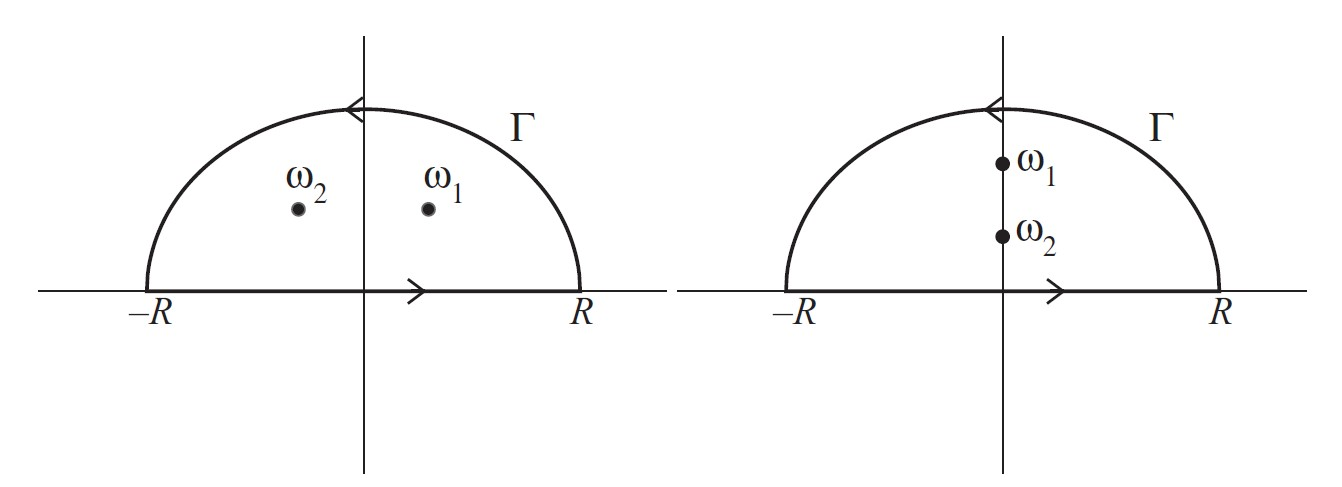
\includegraphics[width=\linewidth]{Lectures/Images/poles.jpg}
    \caption{The two poles have a different
location in the underdamped case (left) and in the overdamped case (right), but they are always in the upper-half
complex plane, therefore preserving causality.}
    \label{fig:poles}
\end{figure}

There are no poles in the lower half plane and that has to do with the constraint given by \textit{causality}, which states that $G(t)\overset{!}{=}0$ for $t<0$. \\

We can obtain an explicit expression of $G(t)$ for $t>0$ by considering the inverse Fourier transform of $G(\omega)$:
\begin{equation}
G(t)=-\frac{1}{2 \pi} \int_{-\infty}^{+\infty} d \omega e^{i \omega t} \frac{1}{m\left(\omega-\omega_{1}\right)\left(\omega-\omega_{2}\right)}
\label{eq:integ}
\end{equation}

Now we will use the residues theorem and we will compute integral (\ref{eq:integ}) over the real line using the fact that we can consider an integral over the circuit represented in Figure \ref{fig:poles}:
\begin{equation}
G(t)=-\frac{1}{2 \pi m} 2 \pi i\left[\frac{e^{i \omega_{1} t}}{\omega_{1}-\omega_{2}}+\frac{e^{i \omega_{2} t}}{\omega_{2}-\omega_{1}}\right], \,\,\,\,\, \text{with} \,\, \omega_1-\omega_2=2\Omega
\end{equation}

Combining the two exponential factors together in order to obtain a sine function we get:
\begin{align}
    \boxed{G(t)=\frac{\sin (\Omega t)}{m \Omega} e^{-\gamma t / 2}}
\end{align}
This relation is general, even when $\Omega \notin \mathbb{R}$, and we can point out that in the underdamped case that the Green function has an\textit{ exponential decay } with characteristic time $\tau=2/\gamma$ and oscillations with frequency $\Omega$.

In the overdamped case what happes is taht we have no more oscillation because $\Omega$ is now imaginary and then $\omega_{1,2}$ are pure imaginary numbers with positive imaginary part (therefore both terms correspond to an exponential decay with two different characteristic time). \\

In this simple example we realized that the imaginary part of the poles is related to exponential decay, whereas the real part is related to oscillations\footnote{This is a general feature in the properties of response functions.}.

\subsection{Strongly overdamped regime}

If we set the inertial term to zero $m=0$ then the Green function in the frequency domain becomes:
\begin{equation}
    G(\omega)\simeq \frac{1}{k+i\tilde{\gamma}\omega}
    \label{eq:approx}
\end{equation}

and so in this approximation we have just one (imaginary) pole, namely:
\begin{equation*}
    \omega_1=\frac{i k}{\tilde{\gamma}}
\end{equation*}


Let's compute the power spectrum in this simple case  using the approximation (\ref{eq:approx}):
\begin{eqnarray}
C(\omega)=-\frac{2}{\beta \omega} G^{I}(\omega) &=\frac{-2}{\beta\omega} \frac{-\omega \tilde{\gamma}}{K^{2}+\tilde{\gamma}^{2} \omega^{2}}= \\
&=\frac{2}{\beta}\frac{\tilde{\gamma}}{k^2+\omega^2\tilde{\gamma}}^2
\end{eqnarray}

which is a Lorentzian function with width of $k/\tilde{\omega}$. Our power spectrum for the harmonic oscillator in the overdamped regime can be represented as in Figure (\ref{fig:foto}).

\begin{figure}[ht]
    \centering
    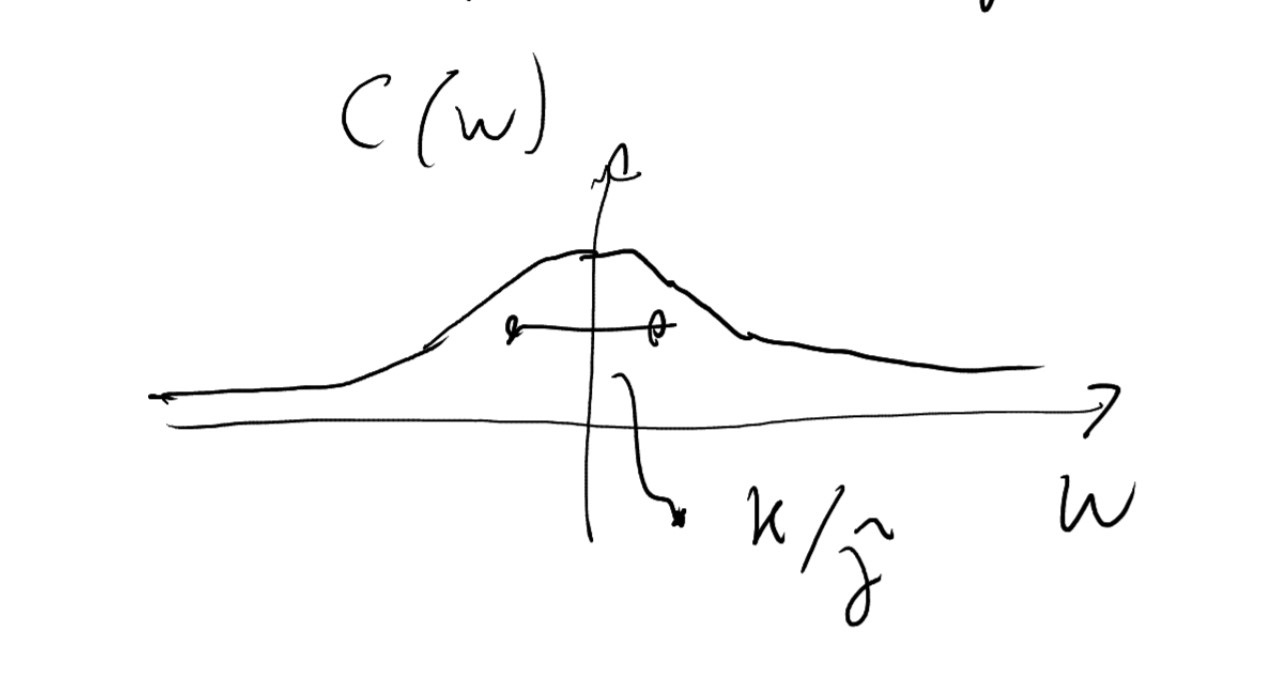
\includegraphics[width=0.5\linewidth]{Lectures/Images/od.jpg}
    \caption{Plot of the overdamped harmonic oscillator power spectrum.}
    \label{fig:foto}
\end{figure}

\end{document}